\documentclass[aspectratio=169,10pt]{beamer}
\usepackage{teaching_slides}


\title{Pass-Through}
\author{C.Conlon}
\institute{Grad IO}
\date{Fall 2026}

\begin{document}

\frame{\titlepage}

\section{What is pass-through and why do we care?}

\begin{frame}{Pass-Through: What is it?}
Lots of cases in economics where we want to know how prices respond to changes in costs:
\begin{itemize}
    \item Response to cost shocks (oil shock, commodity prices)
    \item Response to tax changes (incidence/efficiency of taxes)
    \item Transmission of exchange rate shocks
    \item Transmission of monetary policy
    \item Price effects of mergers: converting \alert{UPP} (a change in opportunity cost) into a change in price
    \item Double marginalization: how much of a wholesale price change reaches the shelf
\end{itemize}
Today: what determines pass-through in theory, what the demand models of this course imply for it, and why it is so hard to estimate.
\end{frame}


\begin{frame}{Hot take}
Pass-through is the simplest thing in economics that nobody understands
\begin{itemize}
\item Often we are talking about different things
\begin{itemize}
\item IO: mostly $\rho = \frac{\partial p_j}{\partial mc_j}$ or the matrix $\frac{\partial\, \symbf{p}}{\partial\, \symbf{mc}}$
\item Macro/Trade: mostly $\frac{\partial \log p_j}{\partial \log mc_j}$
\item (Throughout this lecture $\rho$ is the \alert{pass-through rate} -- not the nesting parameter from the demand lectures.)
\end{itemize}
\item One thing we know for sure: constant marginal costs, perfect competition: \\
 $$p = mc \rightarrow \frac{\partial p}{\partial mc} = 1$$
 \item Everything else depends on two things:
\begin{itemize}
\item \alert{Curvature} of demand (second derivatives)
\item Nature of \alert{competition} (conduct)
\end{itemize}
\item Neither is something an own-price elasticity pins down. That is the whole lecture.
\end{itemize}
\end{frame}


\begin{frame}{The Empirical Puzzle: Estimates Are All Over the Place}
\footnotesize
\begin{center}
\renewcommand{\arraystretch}{1.05}
\scriptsize
\begin{tabular}{lll}
\toprule
Shock $\rightarrow$ price & $\widehat{\rho}$ & Source \\
\midrule
Exchange rate $\rightarrow$ US import prices, dollar-priced & 0.25 & Gopinath Itskhoki Rigobon 2010 \\
\quad same, priced in foreign currency & 0.95 & \\
Exchange rate $\rightarrow$ retail beer & $\approx 0.25$ & Goldberg Hellerstein 2013 \\
Commodity (coffee) $\rightarrow$ retail & $\approx 0.30$ & Nakamura Zerom 2010 \\
Cigarette taxes & $<1$ \,/\, $\approx 1$ & Harding et al.\ 2012 / DeCicca et al.\ 2013 \\
Gasoline taxes & $\approx 1$; holidays $\ll 1$ & Marion Muehlegger 2011; Doyle Samphantharak 2008 \\
Sales taxes & $\approx 1$, half $>1$ & Poterba 1996; Besley Rosen 1999 \\
Alcohol taxes & 1.5 -- 2.1 & Young Bielinska-Kwapisz 2002; Kenkel 2005 \\
\bottomrule
\end{tabular}
\end{center}
\footnotesize
\begin{itemize}
\item Trade theory (CES + monopolistic competition) predicts 0 or 1 depending on invoicing currency. The data say 0.25 and 0.95.
\item Anything from 0.25 to 2 shows up. Theory says that is \alert{exactly what to expect}: pass-through is about curvature and conduct, and both vary across markets.
\item Many ``price elasticity'' studies (gasoline, cigarettes, alcohol) assume $\rho = 1$ and regress quantities on tax changes: $\frac{\partial \log q}{\partial \log t} = \frac{\partial \log q}{\partial \log p}$ (!)
\end{itemize}
\end{frame}


\section{One product, one price}

\begin{frame}{Perfect Competition: Jenkin (1872), Alfred Marshall (1890)}
\begin{align*}
D(p) &= S(p-t)\\
\rho&= \frac{d p}{d t} = \frac{1}{1 + \frac{\varepsilon_d}{\varepsilon_s}}
\end{align*}

\begin{itemize}
\item Where $\varepsilon_d$ is \alert{demand elasticity} and $\varepsilon_s$ is \alert{supply elasticity} respectively.\\
\item $\rho \in [0,1]$ as long demand slopes down and supply slopes up!
\item Constant MC implies that $\varepsilon_s \rightarrow \infty$ and $\rho \rightarrow 1$
\item Incidence $I = \frac{\frac{d\, CS}{d\, t}}{\frac{d\, PS}{d\, t}} = \frac{\rho}{1-\rho}$ (higher pass-through, more borne by consumers)
\end{itemize}
So far so good. Nothing about curvature yet: with perfect competition only slopes matter.
\end{frame}


\begin{frame}{Monopoly (Weyl and Fabinger, JPE 2013)}
\footnotesize
Start with $MR = MC$ and differentiate with respect to the tax $t$:
\begin{align*}
p(q) + p'(q)\, q &= mc(q) + t
\quad \Rightarrow \quad \frac{dq}{dt} = \frac{1}{mr' - mc'}
\quad \Rightarrow \quad \rho = \frac{dp}{dt} = p'\frac{dq}{dt} = \frac{p'}{mr' - mc'}
\end{align*}
Define the markup term $ms(q) \equiv -p'(q)\, q$ and the elasticities $\epsilon_D = -\frac{p}{p' q}$, $\epsilon_S = \frac{mc}{mc'\, q}$, $\epsilon_{ms} = \frac{ms}{ms'\, q}$. Using the Lerner index $\frac{mc}{p} = \frac{\epsilon_D - 1}{\epsilon_D}$:
\begin{align*}
\boxed{\;\rho=\frac{1}{1+\frac{\epsilon_D-1}{\epsilon_S}+\frac{1}{\epsilon_{m s}}}\;}
\qquad\text{constant MC: } \rho = \frac{1}{1 + 1/\epsilon_{ms}}, \qquad
\frac{1}{\epsilon_{m s}}= 1+\frac{p^{\prime \prime} q}{p^{\prime}}
\end{align*}
\begin{itemize}
\item $\epsilon_D > 1$ for a monopolist (except for my MBA students).
\item $1/\epsilon_{ms}$ is the \alert{curvature} of (inverse) demand, and $(\log D)'' = -\frac{1}{\epsilon_{ms}} \frac{1}{ms^2}$, so its sign is the sign of the curvature of \alert{log demand}:
\begin{itemize}
\item log-concave demand $\Rightarrow 1/\epsilon_{ms} > 0 \Rightarrow \rho < 1$ (linear demand: $\rho = 1/2$)
\item log-linear (exponential) demand $\Rightarrow \rho = 1$
\item log-convex demand $\Rightarrow \rho > 1$ (constant elasticity)
\end{itemize}
\item Bulow and Pfleiderer (1983): with constant MC a monopolist's pass-through is \alert{entirely} about curvature.
\end{itemize}
\end{frame}


\begin{frame}{Canonical Demand Curves (single product, constant MC)}
\small
\begin{center}
\renewcommand{\arraystretch}{1.15}
\begin{tabular}{llll}
\toprule
Demand & $\rho = dp/dc$ & $\log D$ & Markup \\
\midrule
Perfect competition & $1$ & -- & $0$ \\
Linear $q = a - b p$ & $1/2$ & concave & $(p - c) = \frac{a - bc}{2b}$ \\
Exponential $q = A e^{-\lambda p}$ & $1$ & linear & $p - c = 1/\lambda$ (constant) \\
Constant elasticity $q = A p^{-\epsilon}$ & $\frac{\epsilon}{\epsilon - 1} > 1$ & convex & $p = \frac{\epsilon}{\epsilon-1} c$ (constant Lerner) \\
Logit, single-product firm, rivals fixed & $1 - \sigma_j$ & concave & $p_j - c_j = \frac{1}{\alpha (1-\sigma_j)}$ \\
\bottomrule
\end{tabular}
\end{center}
\begin{itemize}
\item Linear, exponential and constant-elasticity are the $\rho = \frac{1}{2}$, $1$, $>1$ members of the Bulow--Pfleiderer (1983) constant pass-through family; the puzzle slide lives between the linear and CES rows.
\item A \alert{constant absolute markup} (exponential) gives $\rho = 1$; a \alert{constant percentage markup} (CES) gives $\rho > 1$ because the markup scales with cost. Hence CES trade models over-shift unless pricing-to-market or invoicing is added.
\item Logit sits below one and gets \alert{closer} to one as the product gets smaller. Derivation in two slides.
\end{itemize}
\end{frame}


\begin{frame}{Conduct and Incidence (Weyl and Fabinger 2013)}
Generalize to symmetric imperfect competition with a conduct parameter $\theta$: $\theta=0$ (PC), $\theta=1$ (monopoly), $\theta = 1/N$ (symmetric Cournot):
\begin{align*}
\rho=\frac{1}{1+\frac{\theta}{\epsilon_\theta}+\frac{\epsilon_D-\theta}{\epsilon_S}+\frac{\theta}{\epsilon_{m s}}}
\qquad \text{with } \epsilon_\theta \equiv \frac{\theta}{\theta' q} \text{ (how conduct itself changes with quantity)}.
\end{align*}
Incidence follows from pass-through and conduct alone (their ``Principle of Incidence''):
\begin{align*}
\frac{1}{I} = \frac{1}{\rho} - (1-\theta) \quad\Longleftrightarrow\quad I = \frac{\rho}{1 - (1-\theta)\rho}:
\qquad I_{PC} = \frac{\rho}{1-\rho}, \qquad I_{\text{monopoly}} = \rho.
\end{align*}
\begin{itemize}
\item Monopoly: producer surplus falls by exactly $q$ per dollar of tax (envelope theorem), consumer surplus by $\rho\, q$. So $\rho > 1$ means consumers bear \alert{more than the whole tax}.
\item Two sufficient statistics for incidence, $(\rho, \theta)$, neither of which is an elasticity.
\item Not sure how I feel about the revival of the conduct parameter (more in the conduct lecture).
\end{itemize}
\end{frame}


\begin{frame}{Elasticity vs.\ Curvature: Mr\'azov\'a and Neary (AER 2017)}
\footnotesize
Write everything in terms of inverse demand $p(x)$. Two local statistics at any point:
\begin{align*}
\varepsilon(x) \equiv-\frac{p(x)}{x\, p^{\prime}(x)}>0 \quad \text { (elasticity)} \qquad\qquad
\kappa(x) \equiv-\frac{x\, p^{\prime \prime}(x)}{p^{\prime}(x)} \quad \text{(convexity; MN call it } \rho \text{)}
\end{align*}
\begin{align*}
\text{Monopoly, constant MC:}\qquad \frac{d p}{d c}=\frac{1}{2-\kappa} \qquad \Rightarrow \qquad \frac{d p}{d c}-1=\frac{\kappa-1}{2-\kappa}
\end{align*}
\begin{itemize}
    \item Second-order condition: $\kappa < 2$. Over-shifting ($\rho > 1$) iff $\kappa > 1$: demand more convex than exponential.
    \item \alert{Superconvex} demand ($\kappa > 1 + 1/\varepsilon$, more convex than CES at the same elasticity): the proportional markup $p/c$ \emph{rises} with cost. CES is the boundary.
    \item The \alert{demand manifold}: any demand function traces a curve in $(\kappa, \varepsilon)$ space. The elasticity sets the markup, the convexity sets the pass-through, and \alert{knowing one tells you nothing about the other}.
    \item Our problem in one line: demand estimation targets $\varepsilon$; cost-change counterfactuals need $\kappa$, which the functional form supplies for free.
\end{itemize}
\end{frame}


\begin{frame}{Mr\'azov\'a and Neary (2017): The Space of Elasticity and Convexity}
\begin{center}
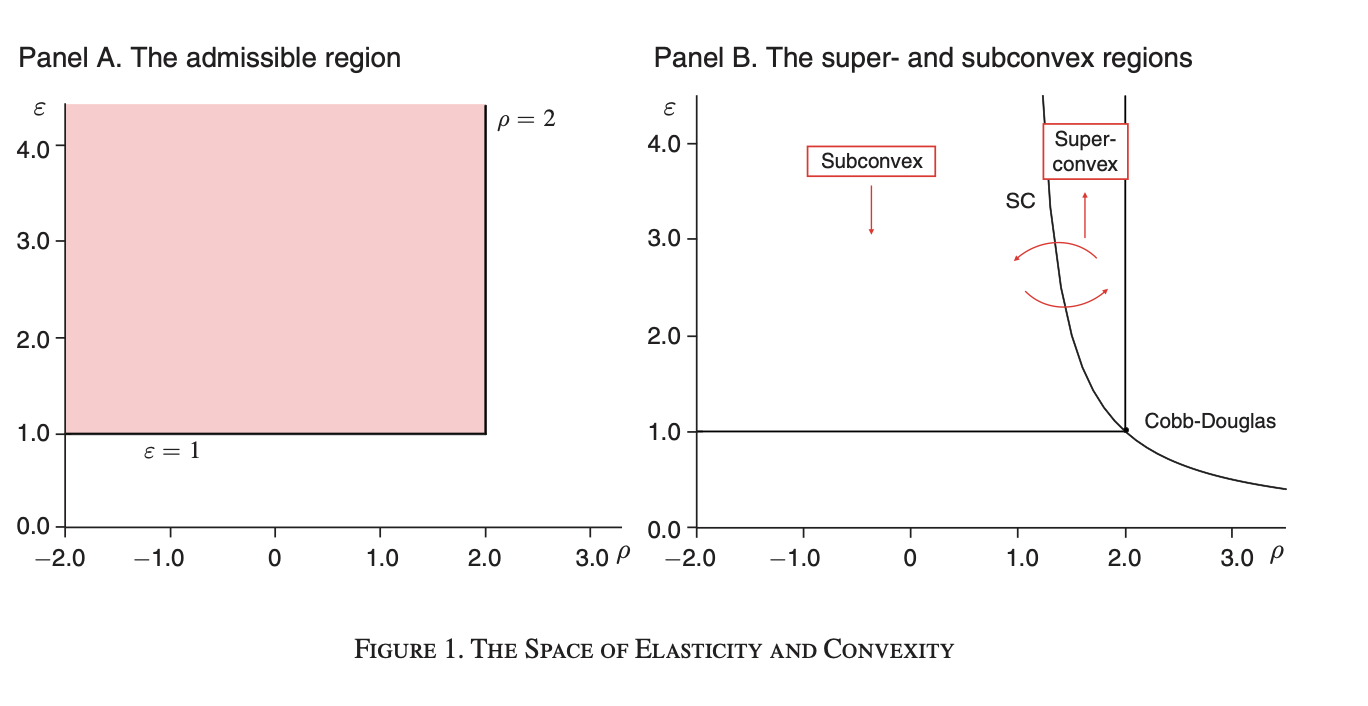
\includegraphics[width=0.72\textwidth]{resources/neary_3}
\end{center}
\vspace{-0.3cm}
{\footnotesize Panel A: the admissible region ($\varepsilon > 1$, $\kappa < 2$). Panel B: the SC curve is the CES family ($\varepsilon$ constant); below it demand is subconvex (proportional markups fall with cost), above it superconvex. Cobb--Douglas is the corner.}
\end{frame}


\section{Discrete choice}

\begin{frame}{Logit Pass-Through in Two Lines}
Single-product firm, plain logit, rivals' prices held fixed. The FOC is $p_j = c_j + \eta_j(p_j)$ with
\begin{align*}
\eta_j = \frac{1}{\alpha (1-\sigma_j)}, \qquad \frac{\partial \eta_j}{\partial p_j} = \frac{1}{\alpha}\frac{1}{(1-\sigma_j)^2}\frac{\partial \sigma_j}{\partial p_j} = -\frac{\sigma_j}{1-\sigma_j}
\qquad \Rightarrow \qquad
\rho_j = \frac{1}{1 - \partial \eta_j / \partial p_j} = \boxed{\;1 - \sigma_j\;}
\end{align*}
\begin{itemize}
\item Logit demand is \alert{log-concave} in own price: $(\log \sigma_j)'' = -\alpha^2 \sigma_j (1-\sigma_j) < 0$, so $\rho_j < 1$ always.
\item The markup $\frac{1}{\alpha(1-\sigma_j)}$ \emph{falls} as the price rises (share shrinks), which is what absorbs part of the cost increase. A niche product passes through almost everything; a dominant product very little.
\item Note what is \alert{not} in the formula: $\alpha$. The price coefficient sets the level of markups and elasticities; the curvature, and hence pass-through, is pinned down by the \alert{share alone}. This is the second-derivative analogue of IIA.
\item With rivals responding (strategic complements) own pass-through is higher and cross pass-through is positive: that needs the matrix (next section). The $1-\sigma_j$ is its ``rivals fixed'' diagonal.
\end{itemize}
\end{frame}


\begin{frame}{Mixed Logit: Curvature Comes From the Mixing Distribution}
\footnotesize
Aggregate demand is a mixture, $\sigma_j(p) = \sum_i w_i\, \sigma_{ij}(p)$, and mixtures of log-concave functions need not be log-concave.
\begin{itemize}
\item Raise $p_j$: the price-sensitive types (high $\alpha_i$) leave first, so the \alert{residual} demand is less elastic than the average. That selection makes $\log \sigma_j$ more convex than any single type's, and $\rho_j > 1$ becomes possible.
\item So in a BLP model pass-through is a byproduct of the \alert{distribution you assumed for $\alpha_i$} (and the characteristics with random coefficients), which estimation on prices and shares barely disciplines. Normal, lognormal, or a two-point $\alpha_i$ can all fit the same elasticities and imply different pass-through.
\item Miravete, Seim, Thurk (2023, ``Elasticity and Curvature of Discrete Choice Demand Models''): map the $(\varepsilon, \kappa)$ pairs each specification can reach in equilibrium. Plain logit and nested logit are a curve; mixed logit is a region whose shape is set by the mixing family, not the data.
\item Practical advice: (a) report the implied pass-through next to the elasticities, it is a cheap diagnostic; (b) if you have cost or tax variation, \alert{use it as a supply moment} (Conlon Rao in the BLP lecture matched observed markups and a tax change for exactly this reason); (c) if your counterfactual is a cost change, the mixing distribution is doing the work, so vary it.
\end{itemize}
\end{frame}


\section{Many products: the pass-through matrix}

\begin{frame}{Multiproduct Bertrand: Pass-Through Is a Matrix}
\small
Recall the FOC in markup form from the merger simulation lecture, $\Omega(\symbf{p}) \equiv \calH \odot \Delta(\symbf{p})$:
\begin{align*}
f(\symbf{p}, \symbf{mc}) \equiv \symbf{p} - \symbf{mc} - \underbrace{\Omega(\symbf{p})^{-1} \symbf{\sigma}(\symbf{p})}_{\symbf{\eta}(\symbf{p})} = 0 .
\end{align*}
The implicit function theorem, with $\partial f/\partial \symbf{mc} = -\mathbb{I}_J$ because costs enter additively:
\begin{align*}
\mathcal{P} \equiv \frac{\partial \symbf{p}}{\partial \symbf{mc}} = -\left(\frac{\partial f}{\partial \symbf{p}}\right)^{-1} \frac{\partial f}{\partial \symbf{mc}}
= \left( \mathbb{I}_J - \frac{\partial \symbf{\eta}}{\partial \symbf{p}} \right)^{-1}, \qquad \mathcal{P}_{(j,k)} = \frac{\partial p_j}{\partial mc_k}.
\end{align*}
\begin{itemize}
\item Diagonal: own-cost pass-through, now including rivals' equilibrium responses. Off-diagonal: a rival's cost shock moves my price (positive under strategic complements).
\item Single-product logit: $\partial \eta_j/\partial p_j = -\sigma_j/(1-\sigma_j)$ on the diagonal; ignoring the off-diagonal terms gives back $1 - \sigma_j$.
\item Multiproduct firms: $\eta_j$ depends on the margins of all sister products, so a cost shock to $k$ moves $p_j$ with no rival response at all.
\item Everything hard is in $\partial \symbf{\eta} / \partial \symbf{p}$: the derivative of a markup is a \alert{second derivative of demand}.
\end{itemize}
\end{frame}


\begin{frame}{How do we get the pass-through matrix?}
Two ways:
\begin{enumerate}
\item Numerically: perturb the marginal cost of each product $k$ in turn and re-solve for equilibrium prices
\begin{align*}
\symbf{p} &=\symbf{mc} + e_k + \Omega(\symbf{p})^{-1} \symbf{\sigma}(\symbf{p})
\end{align*}
(Morrow Skerlos (2011) fixed point, $J$ solves, finite differences; fine for small $J$.)
\item Analytic: differentiate the FOC and apply the implicit function theorem (next slide).\\
See Jaffe Weyl (AEJM 2013), Miller Weinberg (2017, Appendix E), Conlon Rao (2025).\\
\alert{This is what PyBLP does} with \texttt{results.compute\_passthrough}, building the full $J \times J \times J$ demand Hessian (slow, and $J^3$ memory). \texttt{JaxBLP} contracts that tensor with the markups analytically first and never forms it ($J^2 I$ flops; 0.4s vs.\ 3.7s and 31GB on a 636-product market).
\end{enumerate}
\end{frame}


\begin{frame}{Multivariate IFT: The Hard Part}
Differentiate the FOC with respect to $p_l$ to get column $l$ of $\partial f / \partial \symbf{p}$:
\begin{align}
\frac{\partial f(\symbf{p},\symbf{mc})}{\partial p_l} \equiv e_l + \Omega^{-1}(\symbf{p})
\left[  \calH \odot \frac{\partial\, \Delta(\symbf{p})}{\partial\, p_l} \right]
\Omega^{-1}(\symbf{p})\,
\symbf{\sigma}(\symbf{p}) -\Omega^{-1}(\symbf{p})\, \frac{\partial \symbf{\sigma}(\symbf{p})}{\partial p_l}.
\end{align}
The complicated piece is the demand Hessian: a $J \times J \times J$ tensor with elements $(j,k,l)$, $\frac{\partial^2 \sigma_j}{\partial p_k \partial p_l}$, since $\frac{\partial\, \Delta(\symbf{p})}{\partial\, p_l} = -\frac{\partial^2 \symbf{\sigma}}{\partial \symbf{p} \partial p_l}$.
\begin{itemize}
\item Compactly, with markups $\symbf{\eta} = \Omega^{-1}\symbf{\sigma}$: $\frac{\partial f}{\partial \symbf{p}} = \mathbb{I}_J + \Omega^{-1}\left[ T - \frac{\partial \symbf{\sigma}}{\partial \symbf{p}} \right]$ with $T_{(j,l)} = \sum_m \frac{\partial \Omega_{(j,m)}}{\partial p_l}\, \eta_m$. The tensor only ever appears \alert{contracted with the markups}; computing $T$ directly is what makes the closed form cheap.
\item Orientation (as in the pricing lecture): with product-specific $\alpha_{ik}$, read $\Omega = \calH \odot \Delta'$.
\item For (mixed) logit the Hessian is a sum of products of $\sigma_{ij}$'s and $\alpha_i$'s: the ``curvature from mixing'' slide, in matrix form.
\end{itemize}
\end{frame}


\begin{frame}{Application: From UPP to Price Effects (Jaffe Weyl 2013)}
Recall UPP from the antitrust deck: $UPP_j = \Delta c_j + \sum_{k \in \calJ_{g}}  (p_k-c_k) \cdot  D_{jk} (\symbf{p})$ is a change in \alert{opportunity cost}. But how much do we expect prices to rise?
\begin{itemize}
\item Treat the merger as a cost shock and pass it through: $\Delta \symbf{p} \approx \mathcal{P} \cdot \symbf{UPP}$. The first-order approach to merger analysis.
\item That needs the whole $J \times J$ matrix $\mathcal{P}$, which is $J^2$ numbers (again). So people restrict it: diagonal, or $\mathcal{P} = 0.8 \cdot \mathbb{I}_J$, or just the merging firms' own-cost pass-through.
\item Miller, Remer, Ryan, Sheu (2016) simulate mergers under several demand systems and ask how good the approximation is with the full matrix, the diagonal, or only the merging firms' rows (next slide).
\item Which approximations work depends on demand curvature, and curvature is exactly what the approximation is trying to avoid estimating.
\end{itemize}
\end{frame}


\begin{frame}{Miller, Remer, Ryan, Sheu (2016): How Good Is the First-Order Approximation?}
\begin{columns}
\begin{column}{0.5\textwidth}
\centering
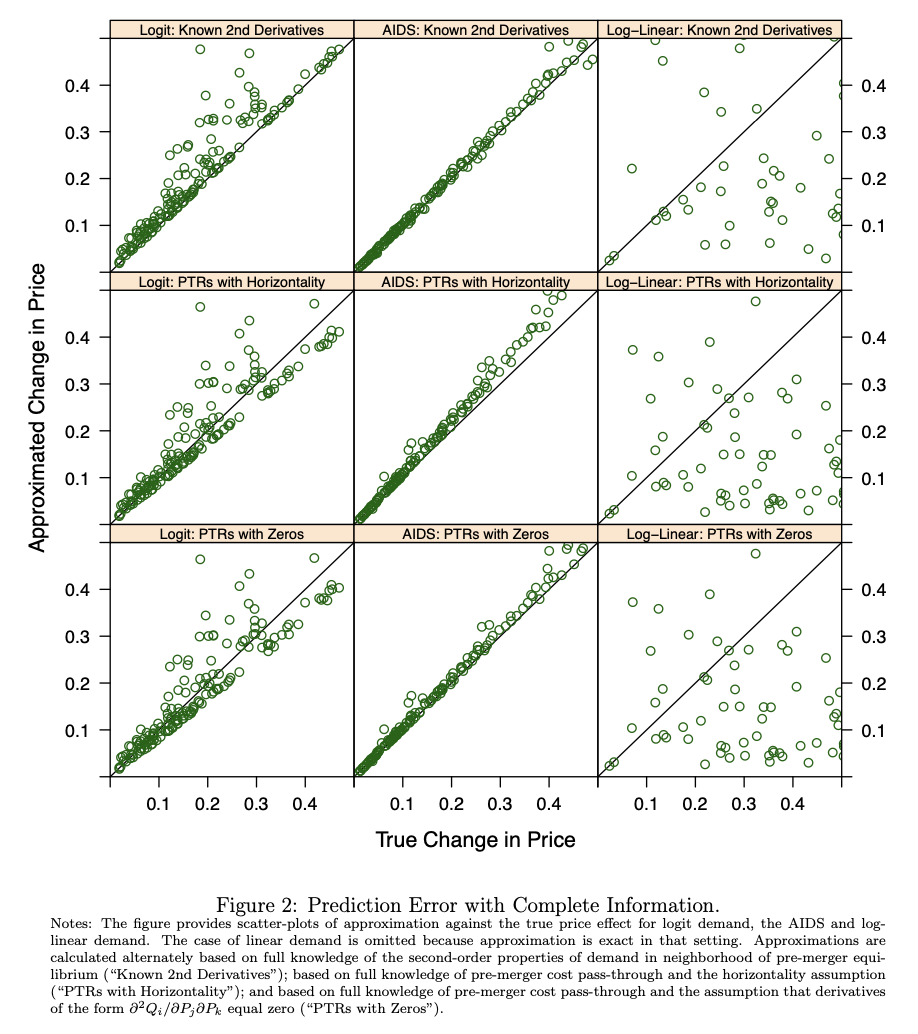
\includegraphics[height=0.66\textheight,width=\textwidth,keepaspectratio]{resources/mrss_complete}
\end{column}
\begin{column}{0.5\textwidth}
\centering
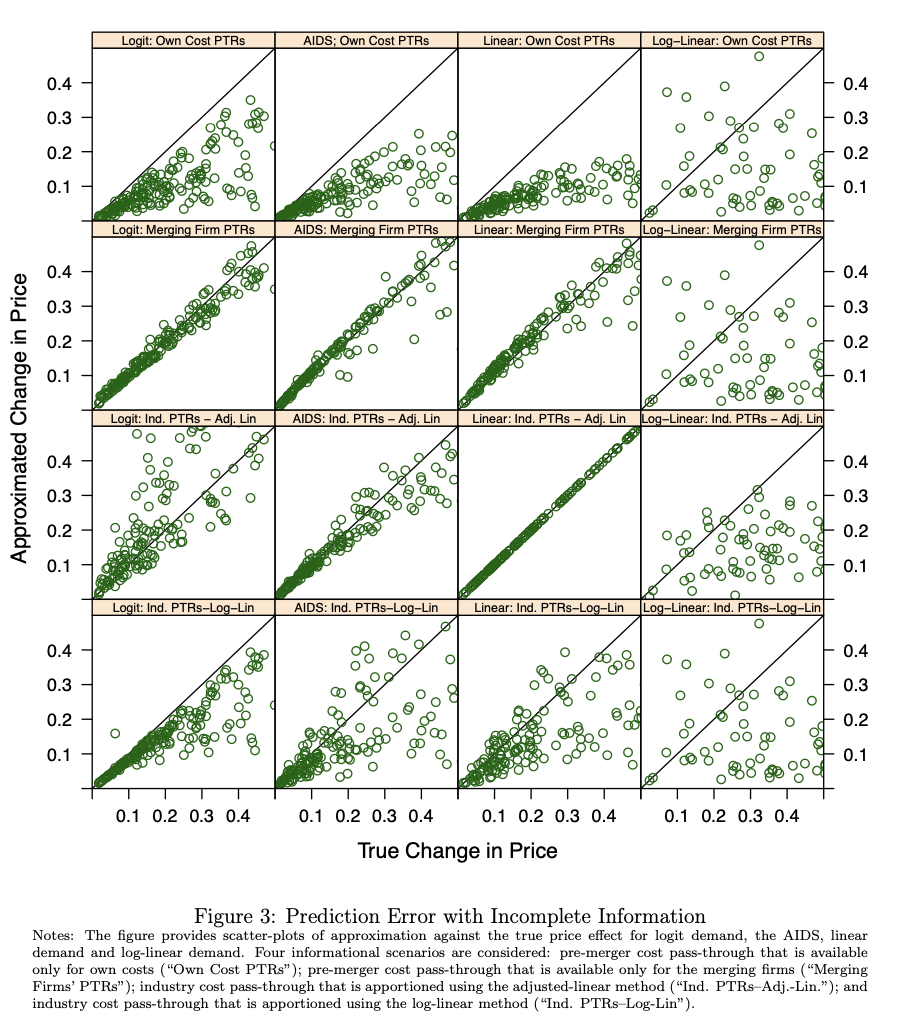
\includegraphics[height=0.66\textheight,width=\textwidth,keepaspectratio]{resources/mrss_incomplete}
\end{column}
\end{columns}
{\footnotesize Left (complete information): with the full pass-through matrix the approximation is close to exact for AIDS and acceptable for logit; log-linear (CES-like) demand is hopeless because the price effect is far from linear in the cost shock. Right (incomplete information): using only own-cost pass-through understates every price effect; the merging firms' rows do most of the work.}
\end{frame}


\section{Vertical chains}

\begin{frame}{Double Marginalization: Villas-Boas (ReStud 2007), Miller Weinberg (Ecma 2017)}
\small
Most retail prices are set by a retailer who buys from a manufacturer with market power. Retailer and wholesaler FOCs:
\begin{align*}
\symbf{p^r} &= \underbrace{\symbf{p^w} +\symbf{c^r}}_{\symbf{mc^r}} +(\mathcal{H}_r \odot \Delta_{r}(\symbf{p^r}))^{-1} \symbf{\sigma}(\symbf{p^r})\\
\symbf{p^w}  &= \symbf{mc^w} + \left(\mathcal{H}_{w} \odot \left( \left[\frac{\partial \symbf{p^r}}{\partial \symbf{p^w}}\right]' \cdot  \Delta_r(\symbf{p^r} ) \right) \right)^{-1} \symbf{\sigma}(\symbf{p^r})
\end{align*}
\begin{itemize}
  \item $\Delta_r$ is the matrix of (retail) demand derivatives with entries $-\frac{\partial\, \sigma_j}{\partial\, p_k^r}$ (as in the merger simulation lecture).
\item $\mathcal{H}_r,\mathcal{H}_w$  ownership matrix $(j,k)=1$ if both products sold by same retailer/wholesaler.
\item $\frac{\partial\, \symbf{p^r}}{\partial\, \symbf{p^w}}$ is the \alert{pass-through matrix} of the retail stage, entry $(m,j) = \partial p^r_m / \partial p^w_j$. Chain rule: $-\partial \sigma_k/\partial p^w_j = \sum_m \frac{\partial p^r_m}{\partial p^w_j} \Delta_{r,(m,k)}$, so the wholesaler's matrix is the \alert{transpose} of the pass-through times $\Delta_r$ (easy to get wrong in code).
\end{itemize}
Challenge: We want $\symbf{p^r}(\symbf{p^w})$ and $\symbf{mc^w}$ but we only have an implicit solution for the retailer FOC. The pass-through matrix is the object that lets the upstream firm's problem be written at all.
\end{frame}


\begin{frame}{Pass-through Counterfactuals? (Conlon Rao 2025)}
\footnotesize
How do we solve for $\symbf{p^w}$ under a counterfactual pass-through matrix?
\begin{itemize}
\item Idea: pass-through only augments the matrix $\Delta_r(\symbf{p^r})$: $\Omega_w \equiv \mathcal{H}_{w} \odot \left( \mathcal{P}' \Delta_r \right)$ with $\mathcal{P} \equiv \frac{\partial \symbf{p^r}}{\partial \symbf{p^w}}$.
\item Example: a constant retail markup or sales tax, $\mathcal{P} = \text{diag}(1+\tau_r)$, so $\mathcal{P}' = \mathcal{P}$ and $\mathcal{P}' \Delta_r = \mathcal{P}\Lambda - \mathcal{P}\Gamma$ with $\mathcal{P}\Lambda$ still diagonal.
\end{itemize}
\begin{align*}
\symbf{p^w}  &= \symbf{mc^w} + \Omega_w^{-1} \symbf{\sigma}(\symbf{p^r})
\end{align*}
Adapt the Morrow Skerlos $\zeta$ fixed point (same sign convention as the pricing lecture, $\alpha_i > 0$). For diagonal $\mathcal{P}$, $\mathcal{H}_w \odot (\mathcal{P}\Gamma) = \mathcal{P}(\mathcal{H}_w \odot \Gamma)$, so $\mathcal{P}$ cancels out of the $\Gamma$ term and survives only on the share term:
\begin{align*}
\symbf{p^w} &\leftrightarrow \symbf{mc^w}+\symbf{\zeta}\left(\symbf{p^w}\right) \quad \text{where}\quad
 \symbf{\zeta}\left(\symbf{p^w}\right)=\Lambda^{-1}\left[\mathcal{H}_w \odot  \Gamma\right]\left(\symbf{p^w}-\symbf{mc^w}\right)+\Lambda^{-1} \alert{\mathcal{P}^{-1}} \symbf{\sigma}
\end{align*}
with $\Lambda, \Gamma, \symbf{\sigma}$ evaluated at $\symbf{p^r}(\symbf{p^w})$. Higher retail pass-through (bigger $\mathcal{P}$) shrinks the wholesale markup: the wholesaler's own price moves retail prices more than one-for-one.
\begin{itemize}
\item General (non-diagonal) $\mathcal{P}$: $\mathcal{P}'\Lambda$ is no longer diagonal, so the clean split fails. Split instead on $D = \text{diag}(\Omega_w)$, iterate $\symbf{p^w} - \symbf{mc^w} \mapsfrom D^{-1}(D - \Omega_w)(\symbf{p^w} - \symbf{mc^w}) + D^{-1}\symbf{\sigma}$ with no convergence guarantee, or use Newton with the pass-through Jacobian.
\end{itemize}
\end{frame}


\begin{frame}{What's the point? Vertical settings}
Why do we care about pass-through in vertical settings?
\begin{itemize}
\item The wholesaler's effective demand derivative is $\mathcal{P}' \Delta_r$: with low retail pass-through the manufacturer faces a flatter response and takes a bigger margin; with high pass-through the retailer is doing the marking up.
\item When retail pass-through is high we think that downstream firms have significant market power.
\item This also means the scope for \alert{elimination of double marginalization} is large.
\begin{itemize}
\item Higher pass-through should be associated with more efficient vertical mergers? (Not sure this has been tested)
\end{itemize}
\item A huge class of models (post-and-hold, minimum markups, RPM, vertical contracts in the second IO course) adds an extra parameter between wholesale and retail prices. All of them are a statement about $\mathcal{P}$.
\end{itemize}
\end{frame}


\section{Taxes and the data}

\begin{frame}{Specific vs.\ Ad Valorem Taxes: The $\zeta$ Map Already Told Us}
\small
Producer price $\symbf{p}$, consumer price $\symbf{p^c}$. A \alert{specific} tax $t$ adds to cost; an \alert{ad valorem} tax $\tau$ scales the consumer price, $\symbf{p^c} = (1+\tau)\symbf{p}$, i.e.\ $\mathcal{P} = (1+\tau)\mathbb{I}_J$ on the previous slide:
\begin{align*}
\text{specific:}\quad \symbf{p} - \symbf{mc} - t\symbf{1} &= \Lambda^{-1}[\calH \odot \Gamma](\symbf{p} - \symbf{mc} - t\symbf{1}) + \Lambda^{-1}\symbf{\sigma}\\
\text{ad valorem:}\quad \symbf{p} - \symbf{mc} &= \Lambda^{-1}[\calH \odot \Gamma](\symbf{p} - \symbf{mc}) + \frac{1}{1+\tau}\Lambda^{-1}\symbf{\sigma}
\end{align*}
\begin{itemize}
\item A specific tax leaves the markup equation alone: the firm re-optimizes against a higher cost and pass-through is $\rho$ from before.
\item An ad valorem tax \alert{taxes the markup}: the share term is scaled by $1/(1+\tau)$, so the producer gives up markup before any demand response. For the same revenue, ad valorem gives lower consumer prices under market power (Delipalla Keen 1992; Anderson, de Palma, Kreider 2001 for logit oligopoly).
\item Single-product logit, rivals fixed: specific tax $\rho = 1-\sigma_j$; ad valorem consumer-price pass-through is smaller still.
\item US excise taxes (gasoline, cigarettes, alcohol, the Seattle soda tax) are \alert{specific}; sales taxes are ad valorem. Conlon Rao (2025) compare volume, sales and ethanol taxes on spirits this way.
\end{itemize}
\end{frame}


\begin{frame}{A simple empirical exercise (Conlon Rao, AEJ:EP 2020)}
\begin{itemize}
\item US states tax distilled spirits by volume (a specific tax)
\item We see tax changes in three states (Connecticut, Louisiana, Illinois)
\item Three popular bottle sizes (750mL, 1L, 1.75L)
\item Run a regression at a 3 month difference product by product
\begin{align*}
\Delta p_{j s t}=\rho_{j s t}(\symbf{X}, \Delta \tau) \cdot \Delta \tau_{j t}+\beta \Delta x_{j s t}+\gamma_j+\gamma_t+\epsilon_{j s t}
\end{align*}
\item Only innovation: allow $\rho_{j s t}(\symbf{X}, \Delta \tau) $ to vary by size of tax increase.
\item Prediction from the theory so far: something below one for a logit-like product, around one with constant markups, above one only with very convex demand.
\end{itemize}
\end{frame}


\begin{frame}{Goes horribly wrong}
\begin{columns}
\begin{column}{0.4\textwidth}
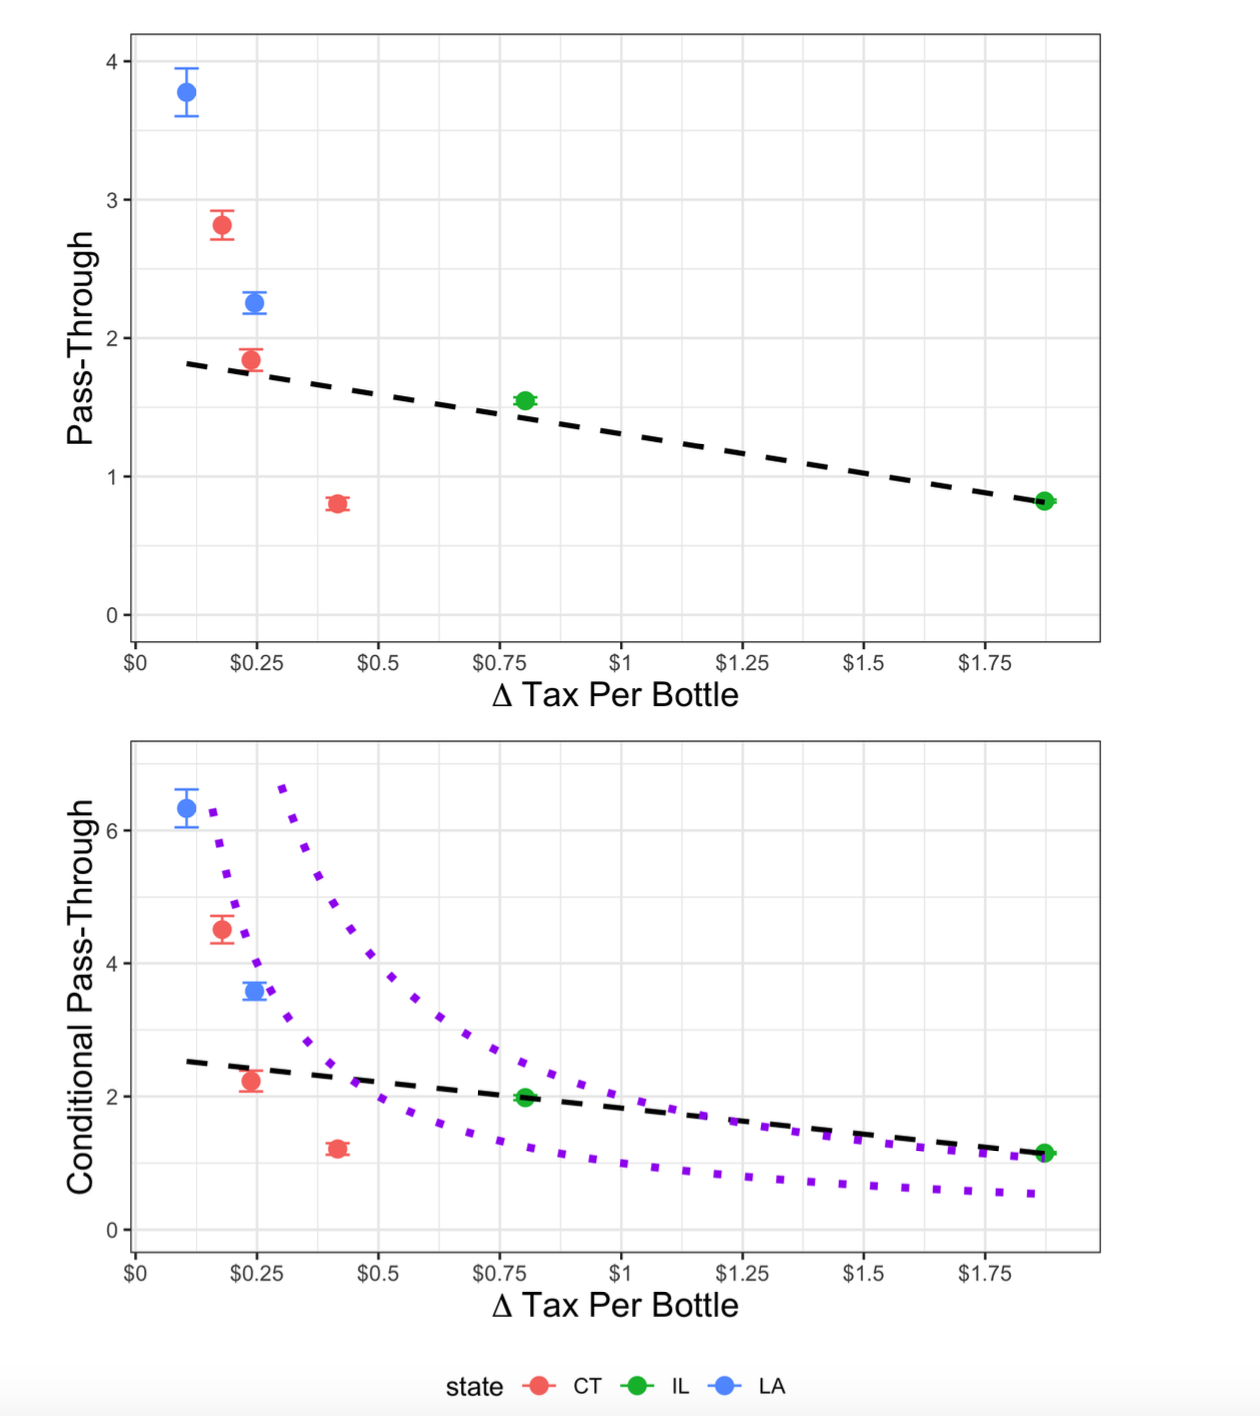
\includegraphics[height=0.9\textheight]{resources/cr_1.png}
\end{column}
\begin{column}{0.5\textwidth}
\begin{itemize}
\item Regression coefficients are huge $>1$ and all over the map
\item Conditional on a price change even larger $>3$
\item Seem to coincide with the purple line
\end{itemize}
\end{column}
\end{columns}
\end{frame}


\begin{frame}{Is PT a structural parameter?}
\begin{columns}
\begin{column}{0.5\textwidth}
\begin{itemize}
\item Price points are a big problem here
\item Estimated an ordered probit with flexible $\beta(\Delta \tau)$
\item Pass-through depends on where you are; not stable at all (!)
\item Maybe structural interpretations of pass-through parameter are a bad idea!
\item The theory is about a smooth FOC. Retail prices move in discrete steps (\$X.99), so a 30 cent tax either does nothing or moves the price a dollar. Averaged over products that can look like anything.
\end{itemize}
\end{column}
\begin{column}{0.5\textwidth}
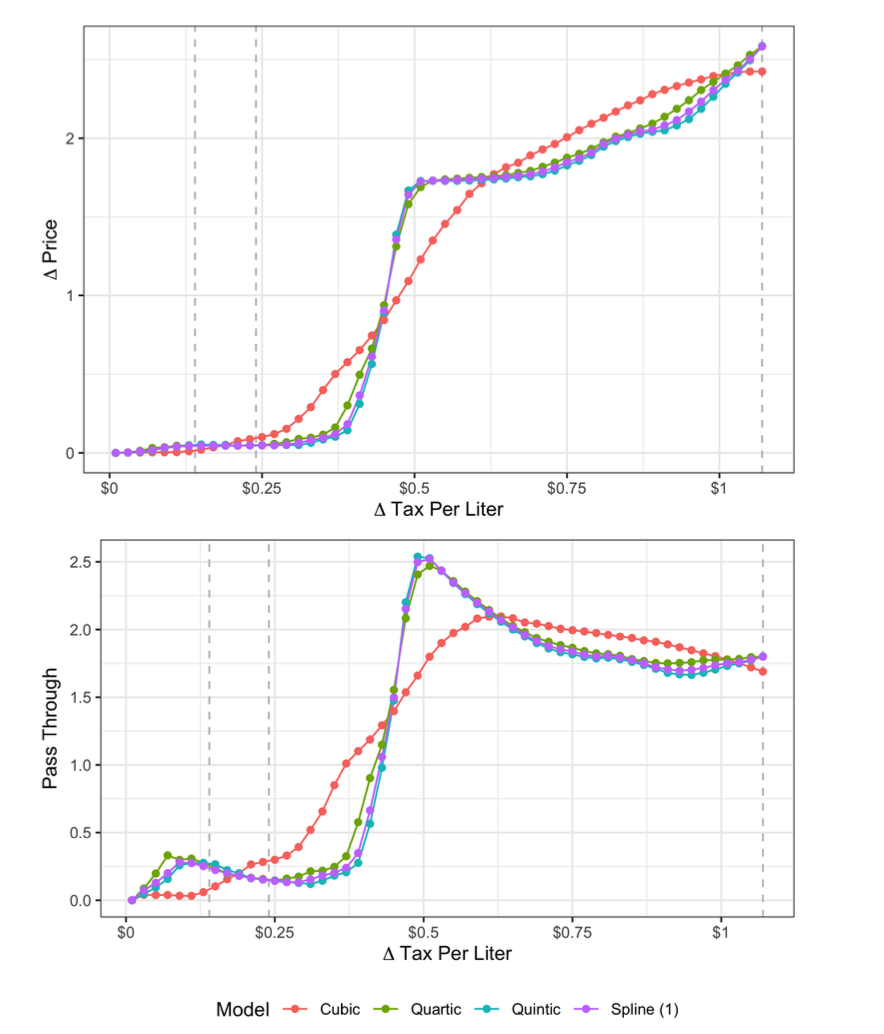
\includegraphics[height=0.9\textheight]{resources/cr_3.png}
\end{column}
\end{columns}
\end{frame}


\begin{frame}{Is It Chain Pricing? DellaVigna Gentzkow (QJE 2019), Butters Sacks Seo (AER 2022)}
\begin{itemize}
\item DellaVigna and Gentzkow (2019): US retail chains set nearly \alert{uniform prices} across their stores despite large differences in local demand and income. So a natural excuse for strange local tax pass-through: the chain prices nationally, the local tax is absorbed or spread across all stores.
\item Butters, Sacks, Seo (2022) test it directly: 68 local excise tax changes (beer, liquor, cigarettes, soda) and 76 sales tax changes, 35,151 stores in 96 multi-state chains.
\begin{itemize}
\item Local cost shocks are passed through to \alert{local} prices, at similar rates for national and local chains.
\item \alert{No spillovers} to unaffected stores in the same chain.
\end{itemize}
\item So chains price uniformly with respect to \alert{demand} but respond locally to \alert{costs}. Uniform pricing is not the explanation for the spirits results; price points and the discreteness of retail pricing are.
\item Practical upshots: (a) local tax changes are clean cost shifters for the supply side of a demand model (the Conlon Rao supply moments); (b) the elasticity you back out from a tax change is the elasticity of the stores that actually changed price, with the price-point weighting from the previous slide.
\end{itemize}
\end{frame}


\begin{frame}{Some challenges}
\begin{itemize}
\item Pless and van Benthem (AEJ:Applied 2019): use pass-through $>1$ as a test for market power? Only if you are willing to rule out convex demand under competition, and to assume constant marginal cost.
\item Chetty, Looney, Kroft (AER 2009)
\begin{align*}
\log q\left(p, \tau^S\right)&=\alpha+\beta \log p+\theta_\tau \beta \log \left(1+\tau^S\right)\\
\theta_\tau&=\frac{\partial \log q}{\partial \log \left(1+\tau^S\right)} / \frac{\partial \log q}{\partial \log p}=\frac{\varepsilon_{q, 1+\tau^s}}{\varepsilon_{q, p}}
\end{align*}
\item Use $\theta$ as evidence of ``tax salience'' (is it?). With imperfect competition the posted price responds to the tax too, so the incidence and excess-burden formulas change: Kroft, Lalibert\'e, Leal-Vizca\'ino, Notowidigdo (ReStud 2024) derive them with salience and market power together, find near-complete pass-through of sales taxes, consumers who respond more to prices than to taxes, and a marginal excess burden larger than the standard formulas give.
\item Can we identify markups from pass-through alone...?!? Only jointly with curvature. Which is where we started.
\end{itemize}
\end{frame}


\end{document}
